\section{PRISM}
\label{sec:prism}
In this section, we introduce \xblue{P}lug-in \xblue{R}emasking for \xblue{I}nference-time \xblue{S}elf-correction of \xblue{M}asked diffusion models (\xblue{\textbf{PRISM}}). We substantiate its theoretical foundation in Section~\ref{sec:prism_theory}, present our empirical modeling design in Section~\ref{sec:prism_empirical}, and explain how PRISM is used during inference in Section~\ref{sec:prism_inference}. Recall the definition of per-token quality from Section~\ref{sec:prior_work_main}:
\begin{equation} \label{def:token_quality}
 g_\star\colon (\mathcal{V}\cup\{\mask\})^L \to [0,1]^L,\quad \xxgreen{g^i_\star(\rvy) \approx (\text{Per-token quality})}=(\text{``how likely'' $\rvy^i$ is given $\rvy$}).
\end{equation}

A natural candidate for the per-token quality is the ground-truth likelihood of the token $\rvy^i$ when $\rvy^i$ is masked out of $\rvy$. We denote this masked sequence by $\rvy\oplus \mask_i$, i.e., $(\rvy\oplus \mask_i)^i=\mask$ and $(\rvy\oplus \mask_i)^j=\rvy^j$ for $j\ne i$.
Our desired notion of \emph{per-token quality} is \coloredhl{xxgreen}{the likelihood of a given token conditioned on the rest of the sequence}. When $\rvy^i$  is consistent with the context $\rvy$, this likelihood should be high; otherwise, it should be low, marking the position as a candidate for remasking. Formally,
\begin{equation*}
    \xxgreen{g_\star^i(\rvy)} := p(\rvx^i = \rvy^i\,|\,\rvy\oplus \mask_i).
\end{equation*}
To clarify, $p(\rvx^i=\cdot \,|\,\cdot)$ is the same as the unmasking posterior used for MDM in Section~\ref{sec:prelim_mdm}.

\textbf{Discussion on our notion of per-token quality.} Since our per-token quality is derived from the posterior, it can be sensitive to uncertainty, e.g., in $\rvy=([\text{I}],\mask,[\text{to}],[\text{school}])$, although the fourth token $[\text{school}]$ is valid, $g_\star^{4}(\rvy)=p(\rvx^4=[\text{school}]\,|\,([\text{I}],\mask,[\text{to}],\mask))$ may be low since there are multiple candidates for that position. In such situations, it cannot ``hurt'' to remask/resample such tokens, as there is high entropy in the true posterior marginal anyway.

More importantly, our notion of per-token quality is effective at detecting \emph{incorrect} tokens in positions with low uncertainty, e.g., in $\rvy=([\text{I}],[\text{eat}],[\text{a}],[\text{apple}], [\text{strudel}])$, the third token $[\text{a}]$ is ungrammatical given $[\text{apple}]$, and $g_\star^{3}(\rvy)$ is sharply concentrated on other words like $[\text{an}]$,$[\text{the}]$; 
our quality score would correctly identify $[\text{a}]$ for remasking and revision.

\textbf{Challenge: Unmasking vs. Remasking training.} Our goal is to train (or obtain) a model $g_\phi$ that approximates $g_\star$. This is challenging because $g_\phi$ must take the sequence where the position $i$ is already unmasked, yet it must approximate the posterior defined with the \emph{masked} context $\rvy\oplus\mask_i$. In contrast, an MDM $f_\theta$ predicts from the masked position itself;
\begin{equation*}
   \xxgreen{g_\phi^i(\rvy)} \approx p(\rvx^i = \rvy^i\,|\,\rvy\oplus \mask_i)\in[0,1],\quad \xblue{f_\theta^i(\cdot \,|\,\rvz)}\approx p(\rvx^i=\cdot\,|\,\rvz)\in\Delta(\mathcal{V}),
\end{equation*}
Although $\xxgreen{g_\phi^i(\rvy)}$ and the $\xblue{f_\theta^i(\cdot\,|\,\rvy\oplus \mask_i)}$'s $\rvy^i$-th coordinate target the same quantity, they condition on different inputs. Consequently, $g_\phi$ cannot be simply trained or efficiently queried as in MDM.

A naive workaround is a distillation-based approach, supervising $\xxgreen{g_\phi^i(\rvy)}$ with the teacher signal $\xblue{f_\theta^i(\cdot\,|\,\rvy\oplus\mask^i)}$. This has two drawbacks: First, even in an infinite data and compute regime, we cannot achieve perfect $g_{\phi^\star}$ if the teacher model $f_\theta$ is imperfect. Second, it is data-inefficient: each training pair $(\rvy,i)$ requires a fresh evaluation of $f_\theta$ on $\rvy\oplus\mask_i$. Consequently, one forward pass of $f$ supervises only a single index, i.e., covering $m$ clean token positions in a sequence requires $m$ passes.

To address this input mismatch, \citet{zhao2024informed} leverage a hollow-transformer $g_{\phi'}$, with the property $g_{\phi'}^i(\rvy\oplus \mask_i)\approx p(\rvx^i=\rvy^i\,|\,\rvy\oplus \mask_i)$, enabling the use of the same loss as MDM. However, this requires adopting a new architecture (with a tweak on the attention mechanism) that processes $\rvy$ while equivalently behaving as if position $i$ were masked, which entails retraining and limiting plug-and-play applicability to pretrained MDMs.

As we will show, PRISM does not possess these limitations: it is plug-and-play with any pretrained MDM $f_\theta$ (no architectural changes), and—even when $f_\theta$ is imperfect, it recovers the desired per-token quality $g_\phi$ in the infinite-data limit.

\subsection{Theoretical foundation of PRISM}\label{sec:prism_theory}
In this section, we establish the theoretical foundation of PRISM. We begin by recalling the premise behind the MDM training loss before describing how we adapt this premise to give rise to PRISM.

\textbf{Marginalization perspective on MDM training.} We rewrite the MDM training loss in~\eqref{eq:unmasking_loss}.
\begin{equation*}
    \mathcal{L}(\theta)\coloneqq  \mathbb{E}_{\rvx,\rvz}\left[\frac{1}{n}\sum_{i\colon \rvz^i=\mask} -\log f_\theta^i(\rvx^i\,|\,\rvz) \right].
\end{equation*}
We now aim to understand why the $\mathcal{L}(\theta)$ has the unmasking posterior as its unique minimizer. First, the expectation over the joint distribution of $(\rvx,\rvz)$ can be written by first sampling $\rvz$ and then $\rvx$ from the induced posterior. For fixed $\rvz$, the loss only depends on the posterior of $\rvx^i$ given $\rvz$, which is exactly the \coloredhl{xblue}{unmasking posterior} $p(\rvx^i=\cdot\,|\,\rvz)$. Thus, we can rewrite:
\begin{equation*}
    \mathcal{L}(\theta) = \mathbb{E}_\rvz \left[\frac{1}{n}\sum_{i\colon \rvz^i=\mask}\xblue{\mathbb{E}_{v\sim p(\rvx^i=\cdot\mid \rvz)}  \left[-\log f_\theta^i(v\,|\,\rvz)\right]} \right],
\end{equation*}
and then we observe that the blue-colored term is the cross-entropy between two distributions $f_\theta^i(\cdot\,|\,\rvz)$ and $p(\rvx^i=\cdot\,|\,\rvz)$, which is minimized at \xblue{$f_{\theta^\star}^i(\cdot\mid \rvz)=p(\rvx^i=\cdot\,|\,\rvz)$} for every $(\rvz,i)$. Put differently, the masking process of MDM defines the joint distribution over $(\rvx,\rvz)$ and fixing $\rvz$ and \emph{marginalizing} over $\rvx$ yields a cross-entropy between the network output and the desired unmasking posterior. We use this marginalization technique to build PRISM.


\textbf{PRISM.} Recall our goal for training $g_\phi$ to predict \coloredhl{xxgreen}{per-token quality}, formally defined as $\xxgreen{g_{\phi^\star}^i(\rvy)=p(\rvx^i=\rvy^i\,|\,\rvy\oplus\mask_i)}$. Given a pretrained MDM $f_\theta$, PRISM proceeds as follows.
\begin{itemize}[leftmargin=17pt, noitemsep, parsep=3pt, topsep=0pt]
    \item[(a)] Construct a pair $(\rvx,\rvz)$ as in MDM training: sample $\rvx\sim p_{\mathrm{data}}$ and then draw $\rvz$ by masking.
    \item[(b)] Sample $\rvy$: choose a masked index $i$ from $\rvz$ and replace it with a clean token $\rvy^i\sim f_\theta^i(\cdot\,|\,\rvz)$.
\end{itemize}
Step (a) defines the same joint distribution over $(\rvx,\rvz)$ as MDM. Step (b) yields a random variable $(\rvy,i)$ conditioned on $\rvz$. Although we do not designate a sampling rule for the index $i$, PRISM's guarantee is invariant to its rule, e.g., uniformly random, confidence-based. As a result, PRISM induces a joint distribution over $(\rvx,\rvz,(\rvy,i))$. Taking expectation over this joint distribution, we define the PRISM loss:
\begin{equation} \label{eq:loss_prism}
    \mathcal{L}(\phi)\coloneqq\mathbb{E}_{\rvx,\rvz, (\rvy,i)}\left[\mathrm{BCE}(\,\mathbf{1}[\rvx^i=\rvy^i]\, , \,\xxgreen{g_\phi^i(\rvy)}\,) \right],
\end{equation}

where $\mathrm{BCE}$ denotes a Binary Cross-Entropy loss  $\mathrm{BCE}(b,p)\!=\!-b\log p \!-\! (1\!-\!b)\log (1\!-\!p)$ for a binary label $b\!\in\!\{0,1\}$. This loss is the crux of PRISM, whose unique minimizer is the true per-token quality.

\begin{tcolorbox}[
  colback=gray!10,
  colframe=black,
  boxrule=0.5pt,
  arc=4pt,
  left=4pt, right=4pt,
  top=1.3pt, bottom=2.0pt,
  boxsep=2.0pt,
  before skip=2.8pt, after skip=2.8pt
]
\begin{proposition}[PRISM] \label{prop:prism_main}
The per-token quality uniquely minimizes the PRISM loss $\mathcal{L}(\phi)$ \eqref{eq:loss_prism}:
\begin{equation*}
g_{\phi^\star}^i(\rvy)=p(\rvx^i=\rvy^i\,|\,\rvy\oplus\mask_i).
\end{equation*}
\end{proposition}
\end{tcolorbox}

Before proving Proposition~\ref{prop:prism_main}, we highlight two key advantages that PRISM offers.

\textbf{Advantages.} First, the minimizer $g_{\phi^\star}^i(\rvy)$ \emph{does not} depend on the specific choice of $f_\theta$; $f_\theta$ affects the training objective only through the marginalized distribution of $(\rvy,i)$, not the minimizer. This contrasts with the aforementioned distillation-based approach, in which an imperfect $f_\theta$ will not give rise to a perfect $g_\phi$. Second, PRISM naturally adapts to a pretrained MDM; a single model can share the same architecture and carry two heads, one for the unmasking posterior and one for per-token quality. We detail the modeling choices of PRISM in Section~\ref{sec:prism_empirical}.

\textbf{PRISM: Guarantee.} Proposition~\ref{prop:prism_main} can be demonstrated within a few lines. The key mechanism is that the joint distribution $(\rvx,\rvz,(\rvy,i))$ exhibits a simple posterior given $(\rvy,i)$; $\rvz$ is deterministically $\rvz=\rvy\oplus\mask_i$ and each $\rvx^i$ is drawn from the same unmasking posterior of MDM, i.e., $v \sim p(\rvx^i=\cdot\,|\,\rvz)$. Therefore, fixing $(\rvy,i)$ and then \emph{marginalizing} the binary label $\mathbf{1}[\rvx^i=\rvy^i]$ over $(\rvx,\rvz)$ yields the simple byproduct,
\begin{equation*}
  \xxpurple{q}\coloneqq\mathbb{E}_{v\sim p(\rvx^i=\cdot \mid \rvy\oplus\mask_i)}\left[\mathbf{1}[v=\rvy^i]\right]= p(\rvx^i=\rvy^i\,|\,\rvy\oplus\mask_i),
\end{equation*}
the per-token quality. We then expand the binary cross-entropy loss:
\begin{align*}
    \mathcal{L}(\phi)=\mathbb{E}_{(\rvy,i)}\left[-\xxpurple{q}\log(\xxgreen{g_\phi^i(\rvy)}) -(\xxpurple{1-q})\log(\xxgreen{1-g_\phi^i(\rvy)}) \right],
\end{align*}
which is exactly minimized at $\xxgreen{g_{\phi^\star}^i(\rvy)=p(\rvx^i=\rvy^i\,|\,\rvy\oplus\mask_i)}$.

\subsection{Empirical design choice of PRISM}\label{sec:prism_empirical}
In this section, we present our empirical modeling choices that go into the design of PRISM. We first explain the plug-and-play aspect of PRISM, in which we adapt a pretrained MDM and fine-tune it via the PRISM loss.
\begin{figure}
  \centering
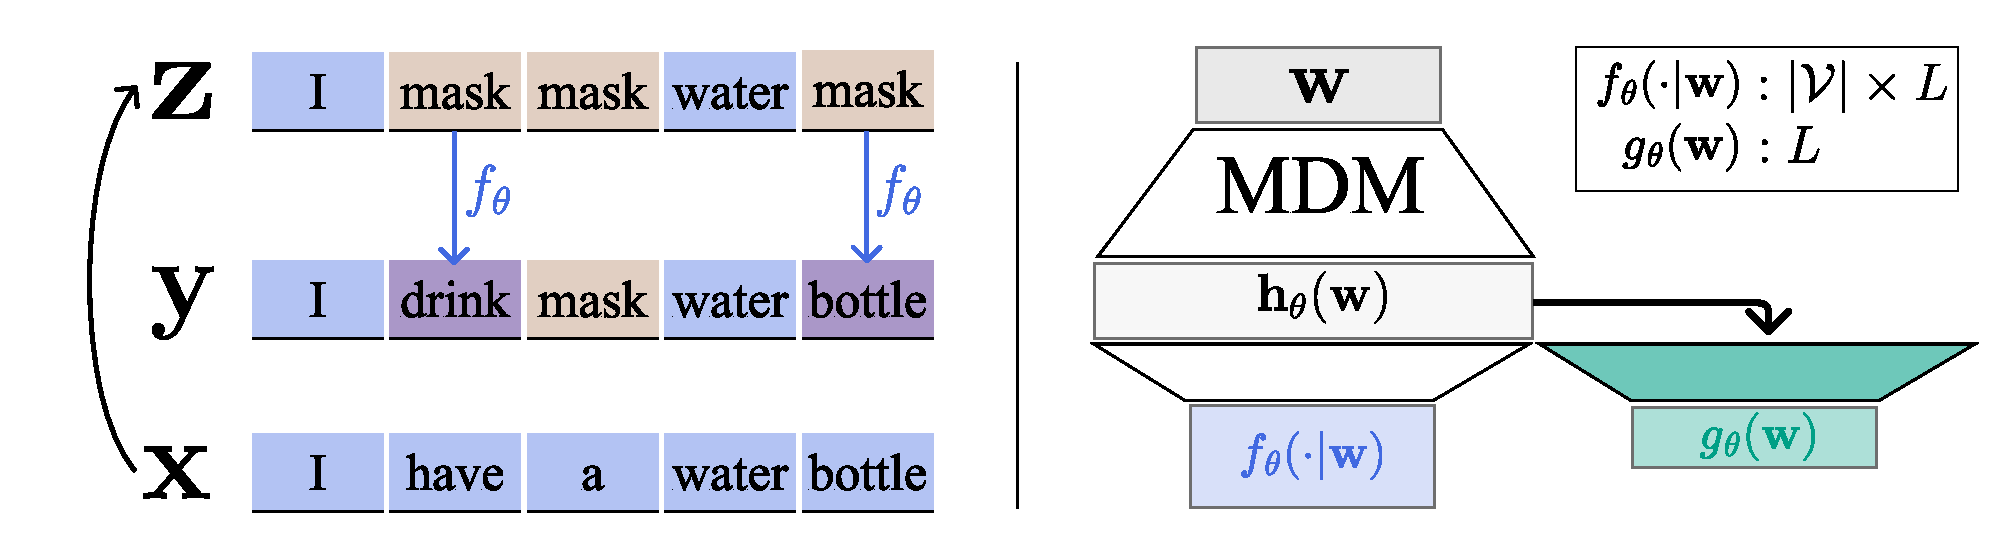
\includegraphics[width=\linewidth,trim={0 0.8cm 0 1.0cm}]{figs/PRISM_pipeline_TK.pdf}
\caption{\textbf{PRISM training pipeline.} Fine-tuning samples are built in two steps; \textbf{(a)} masking process to obtain $(\rvx,\rvz)$ and \textbf{(b)} unmask a few indices in $\rvz$ to get $\rvy$ with a pretrained MDM \xblue{$f_\theta$} (\textbf{Left}). We add a \xxgreen{\emph{lightweight adapter}} to a pretrained MDM so that the resulting model computes the \xblue{\emph{unmasking posterior ($f_\theta$)}} and \xxgreen{\emph{per-token quality} ($g_\theta$)} (\textbf{Right}).}
  \label{fig:prism_training}
   \vskip -\baselineskip
\end{figure}


\textbf{Plug-and-Play approach.} 
Assume a pretrained MDM $f_\theta$ is given, which by design has learned the unmasking posterior. PRISM augments this model with a lightweight auxiliary adapter that reuses the same backbone to produce a size-$L$ tensor. In words, \coloredhl{xxpurple}{the unmasking posterior and per-token quality share a single backbone and are computed by separate heads} (Figure~\ref{fig:prism_training}). 

For a given sequence, we respectively denote the two head outputs as $f_\theta$ and $g_\theta$. Let $\mathbf{h}_\theta$ denote the final hidden state of the MDM backbone. The unmasking posterior $f_\theta$ is obtained by passing $\mathbf{h}_\theta$ through the unmasking head (which originally exists in pretrained MDM) and then applying the softmax. The per-token quality $g_\theta$ is obtained by passing $\mathbf{h}_\theta$ through the attached head and applying the sigmoid. Sigmoid is used to guarantee $g_\theta^i\in[0,1]$, making it suitable for the binary cross-entropy loss. Thus, with a single $\theta$ and a lightweight adapter, we \emph{jointly model} the unmasking posterior and then the per-token quality: for a partially masked sequence $\rvw$,
\begin{equation*}
   \xxgreen{g_\theta^i(\rvw)} \approx p(\rvx^i = \rvw^i\,|\,\rvw\oplus \mask_i)\in[0,1],\quad \xblue{f_\theta^i(\cdot \,|\,\rvw)}\approx p(\rvx^i=\cdot\,|\,\rvw)\in\Delta(\mathcal{V}).
\end{equation*}
At a high level, the PRISM recipe is simple: train $g_\theta$ using the PRISM loss defined in~\eqref{eq:loss_prism}. Consequently, the parameters updated through $g_\theta$ are those of the attached head and the backbone, excluding the unmasking head. As an alternative to fine-tuning the backbone, one can add a LoRA adapter~\citep{hu2022lora} into the backbone and train only the LoRA adapter parameters.

\textbf{Practical interventions.} We introduce two practical interventions that improve PRISM's efficiency. First, to preserve $f_\theta$'s ability to estimate the unmasking posterior while $g_\theta$ is learning toward the per-token quality, we add the MDM training loss~\eqref{eq:loss_prism} as a regularization term. For a regularization constant $\lambda>0$, the total loss is therefore:
\begin{equation} \label{eq:prism_actual_loss}
    \mathcal{L}(\theta) = \mathbb{E}_{\rvx,\rvz, (\rvy,i)}\Bigg[{\mathrm{BCE}(\,\mathbf{1}[\rvx^i=\rvy^i]\, , \,\xxgreen{g_\theta^i(\rvy)}\,)} +  \lambda\times\frac{1}{n} \sum_{j\colon \rvz^j=\mask} \xblue{-\log f_\theta^j(\rvx^j \,|\,\rvz)}\Bigg]. 
\end{equation}
Second, in the sampling process for constructing PRISM training pairs $(\rvx,\rvz, (\rvy,i))$, we modify step (b). To obtain $\rvy$, rather than unmasking a single $\rvy$ from $\rvz$, we obtain multiple $(\rvy,i)$ pairs from one $\rvz$. This produces multiple training pairs $(\rvx,\rvz, (\rvy,i))$ with varying $(\rvy,i)$ values from a single forward pass of $f_\theta(\cdot\,|\,\rvz)$, improving data efficiency. Since this procedure of sample construction minimizes $g_\theta$ (not $f_\theta$), we apply stop-gradient to this $f_\theta$. The pseudocode is given as Algorithm~\ref{alg: adapter fine-tuning}.


\begin{algorithm}[h]
\caption{{PRISM fine-tuning from a pretrained MDM}}
\begin{algorithmic}[1]
\State \textit{Require:} Pretrained MDM backbone \xblue{$f_\theta$}, per-token quality head \xxgreen{$g_\theta$}, optimizer $\mathcal{O}$, true distribution $p_{\mathrm{data}}$, regularization constant $\lambda>0$, number of unmasking tokens $k\in \mathbb{N}$.
    \State Sample $\rvx \sim p_{data}$, $n$, and $\rvz$ from the masking process.
    \State Initialize the loss $\mathcal{L}(\theta) \gets 0$
        \While $\mathcal{L}(\theta)$ converges
        \State \textcolor{gray}{\texttt{\# Sample} $\rvy$ \texttt{from} $\rvz$ \texttt{with} $f_{\mathrm{sg}(\theta)}$}
        \State Select a subset $\mathcal{S} \subseteq \{i \mid \rvz^i=\mask\}$ with $|\mathcal{S}|=k$.
        \State Obtain $\rvy$ by replacing $\rvz^i=\mask$ to  $v^i\sim \xred{f_{\mathrm{sg}(\theta)}^i(\cdot\,|\,\rvz)}$ for each $i\in\mathcal{S}$.
        \State \textcolor{gray}{\texttt{\# Calculate Loss}}
        \State $\mathcal{L}(\theta)\leftarrow \mathcal{L}(\theta)+\frac{1}{|\mathcal{S}|}\sum_{i \in \mathcal{S}}{\mathrm{BCE}(\,\mathbf{1}[\rvx^i=\rvy^i]\, , \,{\xxgreen{g_\theta^i(\rvy)}}\,)}$  \Comment{\textcolor{gray}{PRISM Loss}}
        \State $\mathcal{L}(\theta)\leftarrow \mathcal{L}(\theta)+\lambda \times  \frac{1}{n} \sum_{j:\rvz^j=\mask}\xblue{-\log f_\theta^j(\rvx^j\,|\,\rvz)}$. \Comment{\textcolor{gray}{ Regularization (MDM loss)}}
        \State $\theta \leftarrow \mathcal{O}(\theta, \mathcal{L}(\theta))$
\EndWhile
\end{algorithmic}
\label{alg: adapter fine-tuning}
\end{algorithm}


Importantly, the theoretical guarantee in Proposition~\ref{prop:prism_main} still maintains: the true minimizer $g_\theta$ of this modified PRISM loss continues to encode meaningful per-token quality. We defer the precise statement and proof to Appendix~\ref{proposition_proof}. Moreover, we conduct a careful ablation of different design choices on sampling $\rvy$ in Appendix~\ref{appendix: k_discussion} and Appendix~\ref{appendix:f_theta_discussion}.


\textbf{Practical advantages}. PRISM formulation not only guarantees to minimize the ground truth per-token quality but also has two practical advantages. First, since $f_\theta$ is already pretrained, its hidden states encode useful representations, likely accelerating $g_\theta$'s training on the per-token quality. Second, the targeted per-token quality is a scalar per position, in contrast to the per-position distribution by the unmasking posterior, making it substantially easier to learn. Perhaps surprisingly, we observe that using much less compute compared to MDM pretraining already yields a meaningful learning of the per-token quality (which we detail these results in Section~\ref{sec:experiment}), reinforcing the perspective that PRISM is a cheap \emph{fine-tuning} intervention.

\subsection{Employing PRISM at inference}\label{sec:prism_inference}
In this section, we explain how a model resulting from PRISM is used to perform remasking at inference. The high-level procedure follows Section~\ref{sec:prelim_mdm}; at each inference step, we perform remasking and unmasking simultaneously, using the learned unmasking posterior and per-token quality, respectively.  Assume we are given a fine-tuned MDM $\theta$ (via PRISM loss) and a monotonically decreasing grid of times $t_0=1>\dots>t_N = 0$ for inference. We initialize $\rvx_{t_0}=(\mask,\dots,\mask)$. At each step $t_\ell$, we obtain $\rvx_{t_{\ell+1}}$ by these following steps.
\begin{itemize}[leftmargin=17pt, noitemsep, parsep=3pt, topsep=0pt]
    \item[(a)] Choose a subset of masked tokens $\mathcal{S}$ to \coloredhl{xblue}{unmask}.
    \item[(b)] Choose a subset of clean tokens $\mathcal{T}$ to \coloredhl{xxgreen}{remask} with the lowest quality scores $g_\theta(\rvx_{t_{\ell}})$.
    \item[(c)] For each $i\in\mathcal{T}$, \coloredhl{xxgreen}{remask} $\rvx_{t_\ell}^i$ and for each $j\in\mathcal{S}$, \coloredhl{xblue}{unmask} $\rvx_{t_\ell}^j$ to a clean token sampled from $f_\theta^j(\cdot\,|\, \rvx_{t_\ell})\in\Delta(\mathcal{V})$.
\end{itemize}
We emphasize that $f_\theta^{\cdot}(\cdot\,|\,\rvx_{t_\ell})$ and $g_\theta(\rvx_{t_{\ell}})$ are obtained from a \emph{single} forward pass of the backbone. Consequently, \coloredhl{xxpurple}{our method does not add any computational overhead} relative to methods without remasking (vanilla MDM inference) or training-free approaches, e.g, ReMDM.

\textbf{Design choices.} There are three design choices in this inference procedure: the number of tokens to unmask at each step--$|\mathcal{S}|$, the rule for choosing $\mathcal{S}$, and the number of tokens to remask at each step--$|\mathcal{T}|$. As our focus is on PRISM's remasking strategy, we do not modify the design choices regarding the rule for selecting $\mathcal{S}$ but follow prior seminal approaches. We also keep the rule for selecting $|\mathcal{T}|$ as simple as possible; For unmasking schemes that assign $|\mathcal{S}|$ stochastically, e.g.,~\cite{sahoo2024simple,wang2025remasking,shi2024simplified,gat2024discrete}), $|\mathcal{S}|\sim \mathrm{Binom}(n,p)$ where $p$ depends on the discretized time steps and $n$ is the number of masked tokens in a given sequence. Here we draw $|\mathcal{T}|\sim \mathrm{Binom}(L-n,\eta)$ for $\eta>0$, and accordingly set $|\mathcal{S}|\sim |\mathcal{T}|+\mathrm{Binom}(n,p)$ to preserve the total unmasked count's expectation. For schemes that preallocate $|\mathcal{S}|$s uniformly before inference, e.g.,~\cite{nie2025large}), we likewise preallocate $|\mathcal{T}|$ uniformly across the time steps.